\documentclass{article}

% NIPS style
\usepackage{nips12submit_e, times}

% figures
\usepackage{graphicx}
\graphicspath{{fig/}}

% links
\usepackage[hidelinks]{hyperref}

% better tables
\usepackage{booktabs}
\usepackage{multirow}
\newcommand{\ra}[1]{\renewcommand{\arraystretch}{#1}}


\title{Semi-Supervised Recursive Autoencoders}


\author{
Adrian Guthals \\
\texttt{aguthals@cs.ucsd.edu} \\
\And
David Larson \\
\texttt{dplarson@ucsd.edu} \\
}

\newcommand{\fix}{\marginpar{FIX}}
\newcommand{\new}{\marginpar{NEW}}

% don't show line numbers
\nipsfinalcopy 


\begin{document}

\maketitle


\begin{abstract}
We evaluate semi-supervised recursive autoencoders (RAE) as a method for predicting the sentiment of sentences. Using random word initialization, we are able to predict the sentiment of a movie review dataset with a 74.5\% accuracy, which is only 3.3\% less than the 76.8\% accuracy reported in the 2011 paper ``Semi-Supervised Recursive Autoencoders'' by Soch et al.
\end{abstract}



%-----------------------------------------------------------------------------
% INTRO
%-----------------------------------------------------------------------------
\section{Introduction}

Socher et al. presented a semi-supervised method for learning meanings of sentences using recursive autoencoders \cite{Socher}.

The lecture notes state blah \cite{CSE250B}.

Mention: neural networks, sentence meaning/sentiment



%-----------------------------------------------------------------------------
% ALGORITHMS
%-----------------------------------------------------------------------------
\section{Recursive Autoencoders}

RAE, neural networks, backpropogation, error functions, greedy algorithm, calculating derivatives numerically using finite center-difference


\subsection{Error Function}
\begin{equation}
    E_1 (k) =
\end{equation}

\begin{equation}
    E_2 (k) =
\end{equation}


\subsection{Binary Tree Construction}


\subsection{Backpropogation}
Backpropogation is an efficient method for computing the derivatives required for training a neural network. Given



\subsection{Goal of Training}


\subsection{Gradient Verification}
It is important to verify the accuracy of the gradients calculated using backpropogation. For this study we have chosen to verify the accuracy of backpropogation by comparing against gradients calculated numerically using finite central-differences:
\begin{equation}
    \frac{\partial J}{\partial \theta} = \frac{J(\theta + \epsilon) - J(\theta - \epsilon)}{2\epsilon} + O(\epsilon ^2)
\end{equation}
where $\epsilon$ is the grid spacing.

A downside to using numerical derivatives to verify backpropogation is time complexity. If $W \in R^{2d \times d}$ then the time complexity of computing derivatives is $O(d^2)$ using backpropgation and $O(d^4)$ using finite central-differences, which is not feasible for real-world applications. One option for reducing the time complexity of checking the derivatives is to check a subset of the derivatives, chosen randomly, and assume those selected derivatives are representative of the entire set.


%-----------------------------------------------------------------------------
% EXPERIMENTS
%-----------------------------------------------------------------------------
\section{Experiments}

%
% DATASETS
%
\subsection{Datasets}
We use the same movie reviews dataset as in \cite{Socher}, which consists of 10662 snippets from reviews posted to the Rotten Tomatoes website\footnote{\url{http://www.rottentomatoes.com}}. Each snippet is roughly equivalent to a single sentence and includes a positive/negative label, with the entire dataset containing 5331 positive and 5331 negative labelled snippets. For all experiments we randomly selected $\sim 90\%$ of the original dataset as a training set, with the remaining $\sim 10\%$ used as a testing set. In splitting the dataset we have taken care to prevent any snippets from existing in both sets, so as to not contaminate the results.


%
% OPTIMIZATION
%
\subsection{Optimization}
We use limited-memory Broyden-Fletcher-Goldfarb-Shanno (L-BFGS), a well-known quasi-Newton optimization method, to learn the parameters $\theta$. Specifically we use the Matlab-based L-BFGS function from the minFunc toolbox \cite{minFunc}.


Convergence: error less than $10^{-6}$ (as stated in the project description)

Regularization: ?


%
% RAE
%
\subsection{Experiment 1: RAE}
The full method (RAE)

d = 20: prediction accuracy = 74.5\%

10-fold cross validation

same hyperparameters as Socher et al.




%
% ANALYSIS
%
\subsection{Results}

\subsubsection{Most Positive and Negative}
Table \ref{tab:words}--\ref{tab:phrases} shows the words and phrases predicted to be the most positive and negative. The only result that stands out as possibly an error is the word ``flaws'' being predicted as positive rather than negative. Although the word ``flaws`` may be normally associated with a negative meaning, it could be associated with a positive meaning due its usage in a phrase, e.g., ``despite its flaws''.


\begin{table}[t]
    \centering

    \caption{Words predicted to be the most positive and negative.} 
    \label{tab:words}

    \ra{1.2}
    \begin{tabular}{@{} l l l @{}}
        \\
        \toprule
        \bf{Ranking} & \bf{Positive} & \bf{Negative} \\
        \midrule
        1 & beautiful   & fails  \\
        2 & brilliant   & boring \\
        3 & thoughtful  & neither\\
        4 & triump      & bad \\
        5 & flaws       & flat \\
        6 & beautifully & predictable \\
        7 & success     & bore \\
        8 & spectacular & poorly \\
        9 & enjoyable   & suffers \\
        10 & wonderful  & unnecessary \\
        \bottomrule
    \end{tabular}
\end{table}


\begin{table}[t]
    \centering

    \caption{Phrases (length 2) predicted to be the most positive and negative.} 
    \label{tab:phrases}

    \ra{1.2}
    \begin{tabular}{@{} l l l @{}}
        \\
        \toprule
        \bf{Ranking} & \bf{Positive} & \bf{Negative} \\
        \midrule
        1 & moving and      & lack of \\
        2 & an enjoyable    & boring .\\
        3 & and beautifully & how bad \\
        4 & a moving        & the dullest \\
        5 & a triumph       & flat , \\
        6 & a beautiful     & of bad \\
        7 & the best        & it fails \\
        8 & and powerful    & it isn't \\
        9 & its flaws       & and predictable \\
        10 & a wonderful    & a boring \\
        \bottomrule
    \end{tabular}
\end{table}


\subsubsection{Similar Meanings}
Comparing words and phrases with the most similar meanings is another intiutive method for evaluating the trained model. The similarity between a pair of words or phrases, with meaning vectors $x$ and $y$, can be quantified using cosine similarity:
\begin{equation}
    \textrm{cosine similarity} (x, y) = \frac{\sum_i x_i y_i}{\sqrt{\sum_i x_i^2} \sqrt{\sum_i y_i^2}}
\end{equation}
which is bounded between $-1$ (opposite in meaning) and $+1$ (same in meaning). Applying this metric to Table \ref{tab:words}--\ref{tab:phrases} we find the following pairs to be most similar:
\begin{enumerate}
    \item Positive words: ``bad'' and ``boring''
    \item Negative words: ``wonderful'' and ``enjoyable''
    \item Positive phrases (length 2): ``how bad'' and ``of bad''
    \item Negative phrases (length 2): ``moving and'' and ``and powerful''
\end{enumerate}


\subsubsection{Tree Structure of Interesting Sentences}
Visually inspecting the tree structure of sentences offers on insight on the strengths and weaknesses of the greedy algorithm. Figure \ref{fig:tree_positive} shows the structure of a positive sentence, which the greedy algorithm correctly determined. Meanwhile Figure \ref{fig:tree_negative} shows the structure of a negative sentence which the greedy algorithm performed poorly. Specifically, the structure should have connected ``right now'' with ``go , girls'' instead of ``the reality drain .''. Incorrectly determine tree structures such shown in Figure \ref{fig:tree_negative} likely caused problems for the RAE model and decreased it's prediction accuracy.


\begin{figure}[h]
\begin{center}
    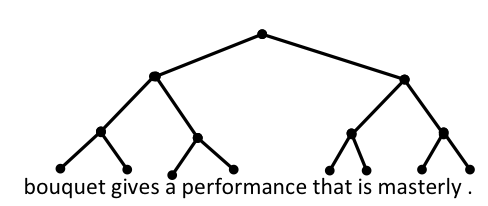
\includegraphics[width=0.7\textwidth]{tree_positive}
    \caption{The tree structured determined by the greedy algorithm of a positive sentence.}
    \label{fig:tree_positive}
\end{center}
\end{figure}


\begin{figure}[h]
\begin{center}
    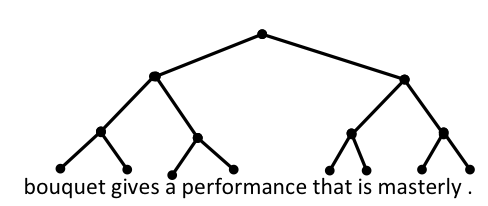
\includegraphics[width=0.7\textwidth]{tree_positive}
    \caption{The tree structured determined by the greedy algorithm of a negative sentence.}
    \label{fig:tree_negative}
\end{center}
\end{figure}




%-----------------------------------------------------------------------------
% CONCLUSION
%-----------------------------------------------------------------------------
\section{Conclusion}
Final remarks



%-----------------------------------------------------------------------------
% BIBLIOGRAPHY
%-----------------------------------------------------------------------------

\small{
\bibliographystyle{IEEEtran}
\bibliography{sources}
}



\end{document}
